\vspace{-6pt}
\subsection{Short-form alignment}
% We first compare baselines and newly developed models on "short-form" test sets. We construct a short-form NOTSOFAR development and test set by dividing the recording into activity-based cuts of at most 30 seconds, with a maximum two-second pause between utterances. We compare our baselines to newly developed models where alignment both with and with out the speaker branch to determine to what extent speaker information improves alignment. As an ablation for the effect of the shuffle graph in alignment, we performed alignment usig the same underlying acoustic model (trained with the shuffle), but we align each individual utterance with ground-truth acoustic boundaries using only the single utterance transcript graph. This experiment isolates the effect of using the shuffle graph for alignment even when the underlying acoustic model is already capable of producing speaker-disentangled output streams. We also evaluate the effect of the long-form tricks from Section \ref{sec:longform_tricks}. Results are shown in Table \ref{tab:baselines_with_average_granular}.
% First we see that all baseline models perform significantly worse than the speaker attributed baseline model from \cite{wiesner2026modeling}, which was a 3-speaker model, unsuitable for evaluation on NSF which has up to 8 speakers. Our new models, which trained on mixtures and scraped data of up to 8 speakers also perform significantly better than the 3-speaker speaker-attributed shuffle model on all dev sets. At least with the additional scraped training data, using a larger number of speakers did not appear to harm performance.

% We see from the Token only row that alignment that ignores the speaker labels slightly degrades performance, but only on the out-of-domain, NSF sets. The row labeled "CTC graph/sup" helps quantify the value of using the shuffle-graph for alignment. the boundary error degrades significantly (104 $\to$ 134 ms) on NSF eval, and results in $50\%$ more swaps on the NSF evaluation set.

% Looking at the long-form tricks, we see that using the 1-state CTC-topology appears to help slightly, presumably because it allows for slightly more flexible alignment than the training topology which forced a blank symbol between every two output tokens. Removing 70\% of the frames predictably degrades performance, but the degradation is very minor, and the resulting speed-up and reduced memory is well worth the performance degradation. Using our lazy graph chunking algorithm does not appear to result in worse alignments. The extra boundary constraints may even help slightly. Finally, BPE trimming improves results significantly. This enables us to train long-form shuffle models more efficiently on larger BPE units while still benefiting from the improved alignments made possible by the finer grain time resolution that smaller units afford. We swept the the max token length parameter for the BPE-trimming from 2-6, and found that using a max length of 4 was optimal.
We first compare baselines and newly developed models on ``short-form'' test sets. We construct short-form NSF development and test sets by dividing recordings into activity-based cuts of at most 30 seconds, with at most two seconds between utterances. We compare alignment with and without the speaker branch to determine whether speaker information improves alignment. To isolate the effect of the shuffle graph, we also align each utterance within its ground-truth acoustic boundaries using the same acoustic model, but only the single-utterance transcript graph. Thus, the model can already produce speaker-disentangled output streams, but alignment does not use the shuffle graph. We also evaluate the long-form tricks from Section~\ref{sec:longform_tricks}. Results are shown in Table ~\ref{tab:baselines_with_average_granular}.

All baseline models perform significantly worse than the speaker-attributed model from~\cite{wiesner2026modeling}, which was limited to three speakers and is therefore unsuitable for NSF, which contains up to eight. Our new models, trained on mixtures and scraped data with up to eight speakers, also outperform the previous model on all development sets, suggesting that increasing the number of speakers does not harm performance with the additional training data. The Token only row shows that ignoring speaker labels degrades alignment, but only on out-of-domain NSF sets. The ``CTC graph/sup.'' row shows that without the shuffle graph BE increases from 104 to 134\,ms and the number of swaps increases by 50\% on NSF eval, 

Among the long-form tricks, the 1-state CTC topology slightly improves alignment, presumably because it is more flexible than the training topology, which forces a blank between output tokens. Removing 70\% of frames causes only minor degradation while substantially reducing computation and memory. Lazy graph chunking also does not degrade alignment, and the additional boundary constraints may help slightly. Finally, BPE trimming improves alignment substantially, allowing efficient training with larger BPE units while retaining the finer temporal resolution of smaller units at inference. Sweeping the maximum BPE token length from 2--6, we found a maximum length of 4 to be optimal.
  \begin{table}[t]
    \centering
    \setlength{\tabcolsep}{2pt}
    \caption{Long-form speaker-attribution performance measured by WDER
    (\%). Chunk-local speaker slots and recording-level speaker identities
    are mapped using oracle permutations.}
    \label{tab:longform_wder}
    \begin{tabular}{@{}l|r|r|r|r@{}}
      \toprule
      Attribution method
        & NSF Dev
        & NSF Eval
        & AMI Dev
        & AMI Test \\
      \midrule
      Segment
        & \textbf{22.0}
        & 32.8
        & \textbf{21.1}
        & \textbf{17.6} \\
      Segment + BPE trim
        & \textbf{22.0}
        & \textbf{32.6}
        & 21.2
        & 17.6 \\
      Word + BPE trim
        & 24.5
        & 35.2
        & 23.9
        & 20.4 \\
        \midrule
        Local Oracle maj. spk & 36.6   &    48.3    &  34.0  &     30.4 \\
    % Global Oracle maj. spk
    % & 58.6 & 63.8 & 64.8 & 60.9 \\
    
      % Random spk / seg
      %   & 69.0
      %   & 68.9
      %   & 70.1
      %   & 69.2 \\
      \bottomrule
    \end{tabular}
    \vspace{-4mm}
  \end{table}

\vspace{-3mm}
\subsection{Long-form Alignment}
\label{sec:results_longform}
We then evaluate these same long-form tricks on the actual long-form NSF recordings, checking what GPU memory and speedups each technique provides. Results are reported in Table \ref{tab:longform_ablation}. First, we notice that there is some small degradation compared to the short-form versions. This is expected as aligning to much longer audio files means alignments have more possibility to drift, early to late, with respect to the reference. We were unable to align using the original training topology so we do not include results here. Since Blank-frame removal is not really compatible with the training topology, which forces blanks between output symbols, we tested the effect of the 1-state topology followed by the blank frame removal. Using all of the long-form alignment tricks resulted in significantly faster alignment and reduced GPU memory.

We also found that BPE trimming interacted very poorly with $\oslash$-removal. Removing up to 40\% of the frames retained the gains of BPE trimming, but removing any more led to significant degradation, even compared to the baseline. Table \ref{tab:longform_ami} extends the most memory efficient long form techniques from Table \ref{tab:longform_ablation} to AMI, which are significantly longer recordings.    


\vspace{-2mm}
\subsection{Speaker Attribution}
In this scenario, we assume transcripts without speaker labels and an oracle map from local to global speaker labels, i.e., perfect clustering to stitch together local diarization results. Table~\ref{tab:longform_wder} shows long-form speaker attribution. WDER is 8.6\% on dev3spk, but degrades considerably on the long-form, out-of-domain AMI and NSF evaluation sets, while remaining well below random chance or majority speaker baselines. One reason is that AMI and NSF segments are considerably shorter: attribution uses non-blank emissions, so dev3spk segments provide multiple pieces of evidence, whereas one-word segments are much more challenging.
\vspace{-2mm}
%% Preamble requirements (add once in the main document):
%   \usepackage{pgfplots}
%   \usepgfplotslibrary{groupplots}
%
% Change this one path if the data directory is stored elsewhere.
\begingroup
\def\aligndatadir{alignment_distribution_data}
% All PGFPlots compatibility and style settings are local to this group.
\pgfplotsset{
  compat=1.17,
  alignment distribution axis/.style={
    width=0.47\textwidth,
    height=0.34\textwidth,
    ymin=0,
    ymax=1.01,
    ylabel={Empirical cumulative probability},
    grid=major,
    grid style={gray!20},
    tick label style={font=\small},
    label style={font=\small},
    title style={font=\small},
    legend style={font=\small, draw=none, fill=none},
  },
  alignment nsf curve/.style={
    blue!70!black, very thick, const plot mark right
  },
  alignment ami curve/.style={
    orange!90!black, very thick, dashed, const plot mark right
  },
}

\begin{figure*}[t]
  \centering
  \begin{tikzpicture}
    \begin{groupplot}[
      group style={group size=2 by 1, horizontal sep=1.15cm},
      alignment distribution axis,
    ]
      \nextgroupplot[
        title={(a) Word-level IoU},
        xlabel={Word IoU (\%)},
        xmin=0, xmax=100,
        legend pos=north west,
      ]
      \addplot[alignment nsf curve]
        table[x=value,y=ecdf] {\aligndatadir/notsofar_eval_word_iou.dat};
      \addlegendentry{NOTSOFAR Eval ($N=41{,}943$ words)}
      \addplot[alignment ami curve]
        table[x=value,y=ecdf] {\aligndatadir/ami_eval_word_iou.dat};
      \addlegendentry{AMI Eval ($N=90{,}149$ words)}

      \nextgroupplot[
        title={(b) Mean IoU per recording},
        xlabel={Recording mean IoU (\%)},
        xmin=50, xmax=75,
        legend pos=north west,
      ]
      \addplot[alignment nsf curve, mark=*, mark size=1.25pt]
        table[x=value,y=ecdf] {\aligndatadir/notsofar_eval_recording_iou.dat};
      \addlegendentry{NOTSOFAR Eval ($N=29$ recordings)}
      \addplot[alignment ami curve, mark=triangle*, mark size=1.5pt]
        table[x=value,y=ecdf] {\aligndatadir/ami_eval_recording_iou.dat};
      \addlegendentry{AMI Eval ($N=16$ recordings)}
    \end{groupplot}
  \end{tikzpicture}
  \caption{Word-level and recording-level distributions of intersection over
  union (IoU). Each recording-level observation is the unweighted mean of the
  word IoUs in one recording. Higher values are better.}
  \label{fig:alignment-iou-distributions}
\end{figure*}

\begin{figure*}[t]
  \centering
  \begin{tikzpicture}
    \begin{groupplot}[
      group style={group size=2 by 1, horizontal sep=1.15cm},
      alignment distribution axis,
    ]
      \nextgroupplot[
        title={(a) Word-level boundary error},
        xlabel={Word boundary error (ms)},
        xmode=log,
        xmin=0.1, xmax=20000,
        legend pos=south east,
      ]
      \addplot[alignment nsf curve]
        table[x=value,y=ecdf] {\aligndatadir/notsofar_eval_word_boundary.dat};
      \addlegendentry{NOTSOFAR Eval}
      \addplot[alignment ami curve]
        table[x=value,y=ecdf] {\aligndatadir/ami_eval_word_boundary.dat};
      \addlegendentry{AMI Eval}

      \nextgroupplot[
        title={(b) Mean boundary error per recording},
        xlabel={Recording mean boundary error (ms)},
        xmin=40, xmax=190,
        legend pos=south east,
      ]
      \addplot[alignment nsf curve, mark=*, mark size=1.25pt]
        table[x=value,y=ecdf]
        {\aligndatadir/notsofar_eval_recording_boundary.dat};
      \addlegendentry{NOTSOFAR Eval}
      \addplot[alignment ami curve, mark=triangle*, mark size=1.5pt]
        table[x=value,y=ecdf] {\aligndatadir/ami_eval_recording_boundary.dat};
      \addlegendentry{AMI Eval}
    \end{groupplot}
  \end{tikzpicture}
  \caption{Word-level and recording-level boundary-error distributions. A
  word's boundary error is the mean of its absolute onset and offset errors;
  each recording-level observation averages that quantity over one recording.
  The word panel uses a logarithmic horizontal axis, with exact zeros displayed
  at $0.1$\,ms. Lower values are better.}
  \label{fig:alignment-boundary-distributions}
\end{figure*}

\begin{figure*}[t]
  \centering
  \begin{tikzpicture}
    \begin{groupplot}[
      group style={group size=2 by 1, horizontal sep=1.15cm},
      alignment distribution axis,
    ]
      \nextgroupplot[
        title={(a) Word-level inversion contribution},
        xlabel={Half inversion degree per word},
        xmode=log,
        xmin=0.01, xmax=30,
        legend pos=south east,
      ]
      \addplot[alignment nsf curve]
        table[x=value,y=ecdf] {\aligndatadir/notsofar_eval_word_kendall.dat};
      \addlegendentry{NOTSOFAR Eval}
      \addplot[alignment ami curve]
        table[x=value,y=ecdf] {\aligndatadir/ami_eval_word_kendall.dat};
      \addlegendentry{AMI Eval}

      \nextgroupplot[
        title={(b) Kendall distance per recording},
        xlabel={Inversions per word},
        xmin=0, xmax=0.5,
        legend pos=south east,
      ]
      \addplot[alignment nsf curve, mark=*, mark size=1.25pt]
        table[x=value,y=ecdf]
        {\aligndatadir/notsofar_eval_recording_kendall.dat};
      \addlegendentry{NOTSOFAR Eval}
      \addplot[alignment ami curve, mark=triangle*, mark size=1.5pt]
        table[x=value,y=ecdf] {\aligndatadir/ami_eval_recording_kendall.dat};
      \addlegendentry{AMI Eval}
    \end{groupplot}
  \end{tikzpicture}
  \caption{Word-level and recording-level ordering-error distributions. Since
  Kendall distance is a sequence statistic, each word receives half the number
  of inversions involving it; its within-recording mean is therefore exactly
  the reported inversions-per-word metric. The word panel uses a logarithmic
  horizontal axis, with exact zeros displayed at $0.01$. Lower is better.}
  \label{fig:alignment-kendall-distributions}
\end{figure*}
\endgroup

%% Preamble requirements (add once in the main document):
%   \usepackage{pgfplots}
%   \usepgfplotslibrary{groupplots}
%
% Change this one path if the data directory is stored elsewhere.
\begingroup
\def\alignmenthistdatadir{alignment_histogram_data}
% All compatibility and style settings are local to this group.
\pgfplotsset{
  compat=1.17,
  alignment histogram axis/.style={
    width=0.47\textwidth,
    height=0.34\textwidth,
    ymin=0,
    ylabel={Fraction of observations},
    grid=major,
    grid style={gray!20},
    axis on top,
    tick label style={font=\small},
    label style={font=\small},
    title style={font=\small},
    legend style={font=\small, draw=none, fill=none},
  },
  alignment nsf histogram/.style={
    ybar interval,
    draw=blue!70!black,
    fill=blue!55,
    fill opacity=0.35,
    line width=0.7pt,
  },
  alignment ami histogram/.style={
    ybar interval,
    draw=orange!90!black,
    fill=orange!70,
    fill opacity=0.35,
    line width=0.7pt,
  },
}

\begin{figure*}[t]
  \centering
  \begin{tikzpicture}
    \begin{groupplot}[
      group style={group size=2 by 1, horizontal sep=1.15cm},
      alignment histogram axis,
    ]
      \nextgroupplot[
        title={(a) Word-level IoU},
        xlabel={Word IoU (\%)},
        xmin=0, xmax=100,
        legend pos=north west,
      ]
      \addplot[alignment nsf histogram]
        table[x=edge,y=probability]
        {\alignmenthistdatadir/notsofar_eval_word_iou.dat};
      \addlegendentry{NOTSOFAR Eval ($N=41{,}943$)}
      \addplot[alignment ami histogram]
        table[x=edge,y=probability]
        {\alignmenthistdatadir/ami_eval_word_iou.dat};
      \addlegendentry{AMI Eval ($N=90{,}149$)}

      \nextgroupplot[
        title={(b) Mean IoU per recording},
        xlabel={Recording mean IoU (\%)},
        xmin=50, xmax=76,
        legend pos=north west,
      ]
      \addplot[alignment nsf histogram]
        table[x=edge,y=probability]
        {\alignmenthistdatadir/notsofar_eval_recording_iou.dat};
      \addlegendentry{NOTSOFAR Eval ($N=29$)}
      \addplot[alignment ami histogram]
        table[x=edge,y=probability]
        {\alignmenthistdatadir/ami_eval_recording_iou.dat};
      \addlegendentry{AMI Eval ($N=16$)}
    \end{groupplot}
  \end{tikzpicture}
  \caption{Normalized histograms of word-level IoU and recording-level mean
  IoU. The two corpora use identical bin edges within each panel. Higher is
  better.}
  \label{fig:alignment-iou-histograms}
\end{figure*}

\begin{figure*}[t]
  \centering
  \begin{tikzpicture}
    \begin{groupplot}[
      group style={group size=2 by 1, horizontal sep=1.15cm},
      alignment histogram axis,
    ]
      \nextgroupplot[
        title={(a) Word-level boundary error},
        xlabel={Word boundary error (ms)},
        xmode=log,
        xmin=0.1, xmax=20000,
        legend pos=north east,
      ]
      \addplot[alignment nsf histogram]
        table[x=edge,y=probability]
        {\alignmenthistdatadir/notsofar_eval_word_boundary.dat};
      \addlegendentry{NOTSOFAR Eval}
      \addplot[alignment ami histogram]
        table[x=edge,y=probability]
        {\alignmenthistdatadir/ami_eval_word_boundary.dat};
      \addlegendentry{AMI Eval}

      \nextgroupplot[
        title={(b) Mean boundary error per recording},
        xlabel={Recording mean boundary error (ms)},
        xmin=40, xmax=190,
        legend pos=north east,
      ]
      \addplot[alignment nsf histogram]
        table[x=edge,y=probability]
        {\alignmenthistdatadir/notsofar_eval_recording_boundary.dat};
      \addlegendentry{NOTSOFAR Eval}
      \addplot[alignment ami histogram]
        table[x=edge,y=probability]
        {\alignmenthistdatadir/ami_eval_recording_boundary.dat};
      \addlegendentry{AMI Eval}
    \end{groupplot}
  \end{tikzpicture}
  \caption{Normalized histograms of word-level and recording-level boundary
  error. A word's boundary error is the mean absolute error of its onset and
  offset; each recording-level observation averages that value over one
  recording. The word-level panel uses logarithmically spaced bins, with exact
  zeros included in the $0.1$\,ms bin. Lower is better.}
  \label{fig:alignment-boundary-histograms}
\end{figure*}

\begin{figure*}[t]
  \centering
  \begin{tikzpicture}
    \begin{groupplot}[
      group style={group size=2 by 1, horizontal sep=1.15cm},
      alignment histogram axis,
    ]
      \nextgroupplot[
        title={(a) Word-level inversion contribution},
        xlabel={Half inversion degree per word},
        xmin=0, xmax=23,
        legend pos=north east,
      ]
      \addplot[alignment nsf histogram]
        table[x=edge,y=probability]
        {\alignmenthistdatadir/notsofar_eval_word_kendall.dat};
      \addlegendentry{NOTSOFAR Eval}
      \addplot[alignment ami histogram]
        table[x=edge,y=probability]
        {\alignmenthistdatadir/ami_eval_word_kendall.dat};
      \addlegendentry{AMI Eval}

      \nextgroupplot[
        title={(b) Kendall distance per recording},
        xlabel={Inversions per word},
        xmin=0, xmax=0.5,
        legend pos=north east,
      ]
      \addplot[alignment nsf histogram]
        table[x=edge,y=probability]
        {\alignmenthistdatadir/notsofar_eval_recording_kendall.dat};
      \addlegendentry{NOTSOFAR Eval}
      \addplot[alignment ami histogram]
        table[x=edge,y=probability]
        {\alignmenthistdatadir/ami_eval_recording_kendall.dat};
      \addlegendentry{AMI Eval}
    \end{groupplot}
  \end{tikzpicture}
  \caption{Normalized histograms of word-level and recording-level ordering
  error. Since Kendall distance is a sequence statistic, each word receives
  half the number of inversions involving it; its mean within a recording is
  exactly the reported inversions-per-word metric. Lower is better.}
  \label{fig:alignment-kendall-histograms}
\end{figure*}
\endgroup

%\begin{table}[t]
\centering
\caption{Long-form inference ablations on NOTSOFAR. RTFx is how much times faster than real time. GPU RAM is in GigaBytes. + BPE trim also uses the lazy graph chunks.}
\label{tab:longform_ablation}
\setlength{\tabcolsep}{1.1pt}
\renewcommand{\arraystretch}{0.92}

\begin{tabular}{@{}l|ccc|ccc|c|c@{}}
\toprule
& \multicolumn{3}{c|}{\textbf{NSF dev}}
& \multicolumn{3}{c|}{\textbf{NSF eval}}
& \textbf{RTFx}
& \textbf{GPU $\downarrow$} \\
\cmidrule(lr){2-4}
\cmidrule(lr){5-7}
\textbf{WavLM 8spk}
& IoU$\uparrow$ & BE$\downarrow$ & $\tau\downarrow$
& IoU$\uparrow$ & BE$\downarrow$ & $\tau\downarrow$
& $\uparrow$ & (GiB) \\
\midrule

+ 1-state topo
& 58.4
& 117
& 12.6
& 58.7
& 104
& \textbf{19.0}
& 9.7 & 14.3 \\

\quad + 30\% frames
& 56.7
& 128
& 12.7
& 57.4
& 111
& 19.2
& 19.3 & 8.5 \\

\qquad + chunks
& 57.4
& 123
& 12.6
& 57.8
& 108
& 19.2
& \textbf{29.8} & \textbf{2.0} \\

\quad + BPE trim
& \textbf{61.0}
& \textbf{112}
& \textbf{12.4}
& \textbf{61.4}
& \textbf{97}
& 19.4
& 17.0 & \textbf{2.0} \\

\bottomrule
\end{tabular}
\vspace{-5mm}
\end{table}
%\begin{table}[t]
  \centering
  \caption{Long-form NOTSOFAR alignment and diarization using the Parakeet
  token-only alignment and token-derived VBx speaker attribution with the
  oracle number of speakers. Calibration offsets were estimated on Dev and
  applied to both timing evaluation and embedding extraction. DER uses
  reference supervision boundaries with a 250\,ms collar.}
  \label{tab:notsofar_parakeet_vbx_calibration}
  \begin{tabular}{llrrrr}
  \toprule
  Set & Calibration
      & Mean IoU $\uparrow$
      & Boundary $\downarrow$
      & WDER $\downarrow$
      & DER $\downarrow$ \\
      & & (\%) & (ms) & (\%) & (\%) \\
  \midrule
  Dev  & None        & 53.9 & 181 & \textbf{28.09} & \textbf{27.27} \\
  Dev  & Dev offsets & \textbf{56.3} & \textbf{176} & 29.28 & 28.10 \\
  \midrule
  Eval & None        & 52.4 & 151 & 42.57 & \textbf{36.87} \\
  Eval & Dev offsets & \textbf{55.0} & \textbf{146} & \textbf{42.05} & 37.24 \\
  \bottomrule
  \end{tabular}
  \end{table}
%\begin{table}[htbp]
\centering
\caption{Parameter sweep over subword \texttt{max length} constraints evaluated on the \texttt{dev3spk} benchmark. BE is measured in milliseconds.}
\label{tab:max_length_sweep}
\begin{tabular}{ccccc}
\toprule
\textbf{max len} & \textbf{avg len} & \textbf{IoU (\%)} $\uparrow$ & \textbf{BE} $\downarrow$ & \textbf{$\tau$  (\%)} $\downarrow$ \\
\midrule
2  & 1.7 & 58.6 & 105 & 34.9 \\
3  & 2.1 & 63.4 & 69  & 16.9 \\
4  & 2.4 & \textbf{64.1} & \textbf{63}  & 12.8 \\
5  & 2.7 & 63.8 & \textbf{63}  & \textbf{12.0} \\
6  & 3.0 & 62.7 & 65  & 12.2 \\
\midrule
\textit{None} & 3.4 & 59.9 & 72  & 13.0 \\
\bottomrule
\end{tabular}
\end{table}
%\begin{table}[htbp]
\centering
\caption{Evaluation results on the \texttt{NOTSOFAR DEV} benchmark showing performance across different percentages of removed tokens at \texttt{max\_length} 4. See Table \ref{tab:max_length_sweep}.}
\label{tab:notsofar_dev_removed}
\begin{tabular}{ccccc}
\toprule
\textbf{Tgt\%} & \textbf{Actual \%} & \textbf{IoU (\%)} $\uparrow$ & \textbf{BE (ms)} $\downarrow$ & \textbf{$\tau$} (\%) $\downarrow$ \\
\midrule
0  & 0.0  & \textbf{60.1} & \textbf{112} & \textbf{12.4} \\
20 & 17.7 & \textbf{60.1} & 113          & 12.5          \\
40 & 32.7 & 60.0          & 115          & 12.5          \\
60 & 48.8 & 57.9          & 129          & 13.0          \\
70 & 58.0 & 56.0          & 146          & 13.5          \\
\bottomrule
\end{tabular}
\end{table}
%\begin{figure}[htbp]
\centering
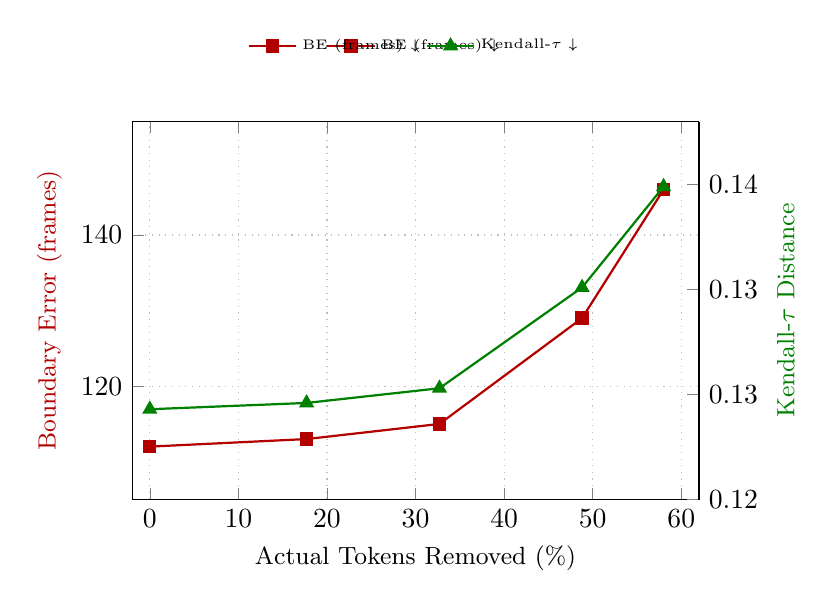
\begin{tikzpicture}
\pgfplotsset{scale only axis}

% -------------------------------------------------------------
% PRIMARY AXIS (Left): Boundary Error (BE)
% -------------------------------------------------------------
\begin{axis}[
    width=7.2cm,
    height=4.8cm,
    xlabel={Actual Tokens Removed (\%)},
    ylabel={Boundary Error (frames)},
    xmin=-2, xmax=62,
    ymin=105, ymax=155,
    axis y line*=left,
    y label style={font=\small, color=red!70!black},
    x label style={font=\small},
    tick label style={font=\xs},
    grid=major,
    grid style={dotted, gray!50},
    legend style={
        at={(0.5, 1.15)},
        anchor=south,
        legend columns=2,
        font=\tiny,
        draw=none,
        fill=none
    }
]

\addplot[color=red!70!black, mark=square*, thick, mark size=2pt] coordinates {
    (0.0, 112)
    (17.7, 113)
    (32.7, 115)
    (48.8, 129)
    (58.0, 146)
};
\addlegendentry{BE (frames) $\downarrow$}

\end{axis}

% -------------------------------------------------------------
% SECONDARY AXIS (Right): Kendall-tau Distance
% -------------------------------------------------------------
\begin{axis}[
    width=7.2cm,
    height=4.8cm,
    xmin=-2, xmax=62,
    hide x axis,
    ylabel={Kendall-$\tau$ Distance},
    ymin=0.120, ymax=0.138,
    axis y line*=right,
    y label style={font=\small, color=green!50!black},
    tick label style={font=\xs},
    legend style={
        at={(0.5, 1.15)},
        anchor=south,
        legend columns=2,
        font=\tiny,
        draw=none,
        fill=none
    }
]

% Legend dummy entry for left-axis metric
\addlegendimage{color=red!70!black, mark=square*, thick, mark size=2pt}
\addlegendentry{BE (frames) $\downarrow$}

\addplot[color=green!50!black, mark=triangle*, thick, mark size=2.4pt] coordinates {
    (0.0, 0.1243)
    (17.7, 0.1246)
    (32.7, 0.1253)
    (48.8, 0.1301)
    (58.0, 0.1349)
};
\addlegendentry{Kendall-$\tau \downarrow$}

\end{axis}

\end{tikzpicture}
\caption{Effect of token pruning rate (\texttt{max\_length}=4) on Boundary Error (BE) and Kendall-$\tau$ distance on the \texttt{NOTSOFAR DEV} benchmark[cite: 5]. Both metrics remain stable up to $\sim 33\%$ actual removal before degradation accelerates[cite: 5].}
\label{fig:notsofar_token_removal}
\end{figure}